\maketitle

\section{编写 LL(1) 语法分析程序}

\subsection{题目要求}

\subsubsection{实验背景}
来自《编译原理与技术(第 2 版)》第 4 章的\textbf{程序设计 2}(方法 2)。

\subsubsection{任务描述}

编写一个 LL(1) 语法分析程序,能对算数表达式进行语法分析。

\paragraph{要求}在给定的消除左递归的文法 $G'$ 的基础上:
\begin{table}[htbp]
    \centering
    \begin{tabular}{@{}ll@{}}
        \toprule
        编号 & 产生式                   \\ \midrule
        1  & $E \to TA $           \\
        2  & $A \to +TA$           \\
        3  & $A \to -TA$           \\
        4  & $A \to ε  $           \\
        5  & $T \to FB $           \\
        6  & $B \to *FB$           \\
        7  & $B \to /FB$           \\
        8  & $B \to \varepsilon  $ \\
        9  & $F \to (E)$           \\
        10 & $F \to \text{num}$    \\
        \bottomrule
    \end{tabular}
\end{table}
\begin{compactenum}
    \item 编程实现算法 4.2,为给定文法自动构造预测分析表。
    \item 编程实现算法 4.1,构造 LL(1) 预测分析程序。
\end{compactenum}

\subsubsection{编程要求}

根据注释提示,补充代码。
\paragraph{要求} 使用 C/C++ 实现

\paragraph{平台环境说明}
\begin{compactitem}
    \item 编译器版本:gcc \texttt{7.3.0}
    \item OS 版本:Debian GNU/Linux \texttt{9}
\end{compactitem}

\subsubsection{测试说明}

\paragraph{输入格式} 从标准输入(使用 \cppinline{cin/scanf} 等输入)读入数据。

输入仅包含 1 行:\begin{compactitem}
    \item 第 1 行输入为一个算术表达式。构成该算术表达式的字符有:\{`\verb|n|', `\verb|+|', `\verb|-|', `\verb|*|', `\verb|/|', `\verb|(|', `\verb|)|' \}。
\end{compactitem}

\paragraph{输出格式} 输出到标准输出(使用 \cppinline{cout/printf} 等输出)中。

输出包括若干行 LL(1) 分析过程:

假设输出有 $n$ 行,则第 $i$ 行 $(1\leq i \leq n)$ 表示分析进行到第 $i$ 步,它的输出包含制表符 (`\verb|\t|') 分隔的三个部分:\begin{compactitem}
    \item 分析栈:以 \verb|$| 符号表示栈底的字符串 (左侧为栈底;由终结符和非终结符构成)
    \item 输入串栈:以 \verb|$| 符号表示栈底的字符串 (右侧为栈底)
    \item 分析动作:产生式编号,或 \texttt{match} 或 \texttt{error} 或 \texttt{accept}(表示当前步骤应执行的动作)
\end{compactitem}

\subsection{程序设计说明}

\begin{compactitem}
    \item \cppinline{prods}:映射产生式编号到(左部, 右部)。
	\item \cppinline{grammar}:记录每个非终结符号的多个产生式右部,用于求 FIRST 和 FOLLOW 集。
	\item \cppinline{FIRSTSets}、\cppinline{FOLLOWSets}:储存每个非终结符号的 FIRST 和 FOLLOW 集。
	\item \cppinline{M}:预测分析表,$M[A][a]$ 给出在 $X$ 为非终结符 $A$ 且当前输入符号为 $a$ 时应选用的产生式编号。
	\item \cppinline{input_line}:存储输入串。
	\item 使用 \verb|@| 表示 $\varepsilon$。
\end{compactitem}

\subsubsection{读入输入串}

在主函数中从标准输入读取一行字符串作为待分析的算术表达式,然后在末尾添加结束符号 \verb|$|。
\begin{cppcode}
    std::string input_line;
    std::getline(std::cin, input_line);
    input_line.push_back('$');
\end{cppcode}

\subsubsection{构建文法}

利用 \cppinline{buildGrammar()} 函数,将产生式存入 \cppinline{grammar} 字典中,并将每条产生式存入 \cppinline{prods} 映射中以便后续查表;同时设置非终结符与终结符集合。
\begin{cppcode}
void buildGrammar()
{
    grammar['E'].emplace_back("TA");
    grammar['A'].emplace_back("+TA");
    grammar['A'].emplace_back("-TA");
    grammar['A'].emplace_back(""); // ε
    grammar['T'].emplace_back("FB");
    grammar['B'].emplace_back("*FB");
    grammar['B'].emplace_back("/FB");
    grammar['B'].emplace_back(""); // ε
    grammar['F'].emplace_back("(E)");
    grammar['F'].emplace_back("n");

    nonterminals = { 'E', 'A', 'T', 'B', 'F' };
    terminals = { 'n', '+', '-', '*', '/', '(', ')', '$' };

    prods[1] = std::make_pair('E', "TA");
    prods[2] = std::make_pair('A', "+TA");
    prods[3] = std::make_pair('A', "-TA");
    prods[4] = std::make_pair('A', "");
    prods[5] = std::make_pair('T', "FB");
    prods[6] = std::make_pair('B', "*FB");
    prods[7] = std::make_pair('B', "/FB");
    prods[8] = std::make_pair('B', "");
    prods[9] = std::make_pair('F', "(E)");
    prods[10] = std::make_pair('F', "n");
}
\end{cppcode}

\subsubsection{求 FIRST 集}

调用 \cppinline{buildFIRST()} 函数,利用 \cppinline{FIRST_str()} 函数为每个非终结符号计算 FIRST 集。其中 \cppinline{FIRST_str()} 用于计算任意符号串的 FIRST 集。\begin{compactitem}
    \item 若首个符号是终结符,FIRST 集即为该终结符本身。
    \item 若首个符号是非终结符,则将该非终结符的 FIRST 集(除 $\varepsilon$ 之外的符号)加入结果中;如果包含 $\varepsilon$,则继续处理下一个符号。
    \item 若最终可推导出 $\varepsilon$,则在 FIRST 中加入 \verb|@|。
\end{compactitem}
重复计算直到 FIRST 集不再变化。
\begin{cppcode}
std::set<char> FIRST_str(const std::string& str)
{
    std::set<char> result;
    if (str.empty()) {
        result.insert('@');
        return result;
    }
    for (int i = 0; i < static_cast<int>(str.size()); i++) {
        char X = str[i];
        if (isTerminal(X)) {
            result.insert(X);
            return result;
        }
        bool hasEpsilon = false;
        for (auto c : FIRSTSets[X]) {
            if (c == '@') {
                hasEpsilon = true;
            } else {
                result.insert(c);
            }
        }
        if (!hasEpsilon) {
            return result;
        }
        if (i == static_cast<int>(str.size()) - 1) {
            result.insert('@');
        }
    }
    return result;
}

void buildFIRST()
{
    bool changed = true;
    for (auto nt : nonterminals) {
        FIRSTSets[nt]; // init empty
    }

    while (changed) {
        changed = false;
        for (auto nt : nonterminals) {
            for (auto& rhs : grammar[nt]) {
                std::set<char> f = FIRST_str(rhs);
                int oldSize = static_cast<int>(FIRSTSets[nt].size());
                for (auto c : f) {
                    FIRSTSets[nt].insert(c);
                }
                if (static_cast<int>(FIRSTSets[nt].size()) > oldSize) {
                    changed = true;
                }
            }
        }
    }
}
\end{cppcode}

\subsubsection{求 FOLLOW 集}

调用 \texttt{buildFOLLOW()} 函数为每个非终结符号计算 FOLLOW 集。\begin{compactitem}
    \item 将 \verb|$| 放入开始符号 $E$ 的 FOLLOW 集。
    \item 对文法中每条产生式 $A \to \alpha B \beta$:
    \item 将 FIRST($\beta$) 除去 $\epsilon$ 加入 FOLLOW(B);
    \item 若 $\beta$ 可推出 $\varepsilon$,则 FOLLOW(A) 中的所有符号也加入 FOLLOW(B)。
\end{compactitem}
\begin{cppcode}
void buildFOLLOW()
{
    for (auto nt : nonterminals) {
        FOLLOWSets[nt];
    }
    FOLLOWSets['E'].insert('$');

    bool changed = true;
    while (changed) {
        changed = false;
        for (auto nt : nonterminals) {
            for (auto& rhs : grammar[nt]) {
                for (int i = 0; i < static_cast<int>(rhs.size()); i++) {
                    char B = rhs[i];
                    if (nonterminals.count(B) != 0U) {
                        std::string beta = rhs.substr(i + 1);
                        std::set<char> firstBeta = FIRST_str(beta);
                        int oldSize = static_cast<int>(FOLLOWSets[B].size());
                        if (firstBeta.count('@') != 0U) {
                            firstBeta.erase('@');
                            for (auto c : firstBeta) {
                                FOLLOWSets[B].insert(c);
                            }
                            for (auto c : FOLLOWSets[nt]) {
                                FOLLOWSets[B].insert(c);
                            }
                        } else {
                            for (auto c : firstBeta) {
                                FOLLOWSets[B].insert(c);
                            }
                        }
                        if (static_cast<int>(FOLLOWSets[B].size()) > oldSize) {
                            changed = true;
                        }
                    }
                }
            }
        }
    }
}
\end{cppcode}

\subsubsection{构造预测分析表 $M$}

求出 FIRST 和 FOLLOW 集后,我们可以方便地构造 LL(1) 分析表,算法如~\autoref{alg:build-predictive-analysis-table} 所示。
\begin{algorithm}[htbp]
    \caption{构造预测分析表 $M$ 的算法}
    \label{alg:build-predictive-analysis-table}
    \KwIn{文法 $G$}
    \KwOut{预测分析表 $M$}

    \ForEach{产生式 $A \to \alpha$ 属于 $G$}{
        \ForEach{$a \in \mathrm{FIRST}(\alpha)$}{
            将 $A \to \alpha$ 加入到 $M[A,a]$ 中\;
        }
        \If{$\epsilon \in \mathrm{FIRST}(\alpha)$}{
            \ForEach{$b \in \mathrm{FOLLOW}(A)$}{
                将 $A \to \alpha$ 加入到 $M[A,b]$ 中\;
            }
        }
    }

    \ForEach{未定义的表项 $M[A,a]$}{
        标记为错误\;
    }

\end{algorithm}

根据算法实现 \cppinline{buildParsingTable()} 函数,根据 LL(1) 文法构造预测分析表 $M$。

对于每个产生式 $A \to \alpha$:\begin{compactitem}
    \item 对 FIRST($\alpha$) 中的每个终结符号 $a$(若非 $\varepsilon$)将 $A \to \alpha$ 填入表项 $M[A, a]$。
    \item 若 $\varepsilon$ 在 FIRST($\alpha$) 中,则对 FOLLOW($A$) 中的每个符号 $b$,将 $A \to \alpha$ 填入 $M[A, b]$。
\end{compactitem}

未定义表项表示 \texttt{error}。
\begin{cppcode}
void buildParsingTable()
{
    for (auto& p : prods) {
        char A = p.second.first;
        std::string alpha = p.second.second;
        std::set<char> firstSet = FIRST_str(alpha);
        bool hasEpsilon = (firstSet.count('@') != 0U);
        for (auto a : firstSet) {
            if (a != '@') {
                M[A][a] = p.first;
            }
        }
        if (hasEpsilon) {
            for (auto b : FOLLOWSets[A]) {
                M[A][b] = p.first;
            }
        }
    }
}
\end{cppcode}

\subsubsection{预测分析}

最后调用 \cppinline{LLparse()} 函数进行 LL(1) 分析。\begin{compactitem}
    \item 初始化分析栈,将 \verb|$| 和开始符号 $E$ 压栈。
    \item 输入串置于输入缓冲区(末尾有 \verb|$|),指针 \cppinline{ip} 指向首符号。
    \item 重复以下步骤直到栈顶为 \verb|$| 并匹配输入 \verb|$|:\begin{compactenum}
              \item 若栈顶 $X$ 为终结符或 \verb|$|:\begin{compactitem}
                        \item 若 $X = a$(当前输入符号),弹栈并前进输入指针 \cppinline{ip};
                        \item 否则报错。
                    \end{compactitem}
              \item 若栈顶 $X$ 为非终结符:\begin{compactitem}
                        \item 查表 $M[X, a]$,若有产生式 $X \to Y_1 Y_2 \dots Y_k$,弹出 $X$,逆序将 $Y_k \dots Y_1$ 入栈;
                        \item 若无匹配产生式则报错。
                        \item 过程中输出分析步骤,包括栈内容、剩余输入串和动作(产生式编号或 \texttt{match}、\texttt{error}、\texttt{accept})。
                    \end{compactitem}
          \end{compactenum}
\end{compactitem}

转化成伪代码如~\autoref{alg:ll1-parsing} 所示。
\begin{algorithm}[htbp]
    \caption{自顶向下预测分析算法}
    \label{alg:ll1-parsing}
    \KwIn{输入符号串 $\omega$,文法 $G$ 的预测分析表 $M$}
    \KwOut{若 $\omega \in L(G)$,则输出 $\omega$ 的最左推导,否则报告错误}

    将 $\$ $ 压入栈底,将文法开始符号 $S$ 压入栈顶\;
        将 $\omega\$ $ 放入输入缓冲区中,并令 $ip$ 指向其第一个符号\;

    \Repeat{$X = \$ $}{
        设 $X$ 为栈顶文法符号,$a$ 为 $ip$ 所指向的输入符号\;
        \If{$X$ 是终结符号或 $\$ $}{
            \If{$X = a$}{
                从栈顶弹出 $X$\;
                将 $ip$ 前移一个位置\;
            }\Else{
                error()\;
            }
        }\Else{
            \If{$M[X,a] = X \to Y_1 Y_2 \cdots Y_k$}{
                从栈顶弹出 $X$\;
                将 $Y_k, Y_{k-1}, \ldots, Y_1$ 依次压入栈,$Y_1$ 位于栈顶\;
                输出产生式 $X \to Y_1 Y_2 \cdots Y_k$\;
            }\Else{
                error()\;
            }
        }
    }
\end{algorithm}

根据伪代码,实现 \cppinline{LLparse()} 函数如下:
\begin{cppcode}
void LLparse(const std::string& input_line)
{
    std::stack<char> st;
    st.push('$');
    st.push(startSymbol);

    int ip = 0;
    bool done = false;
    bool error_flag = false;

    while (!done && !error_flag) {
        char X = st.top();
        char a = input_line[ip];

        if ((terminals.count(X) != 0U || X == '$')) {
            if (X == a) {
                if (X == '$') {
                    printStep(st, input_line, ip, "accept");
                    done = true;
                } else {
                    printStep(st, input_line, ip, "match");
                    st.pop();
                    ip++;
                }
            } else {
                printStep(st, input_line, ip, "error");
                error_flag = true;
            }
        } else {
            if (M[X].find(a) != M[X].end()) {
                int p = M[X][a];
                std::string rhs = prods[p].second;
                printStep(st, input_line, ip, std::to_string(p));
                st.pop();
                for (int i = static_cast<int>(rhs.size()) - 1; i >= 0; i--) {
                    if (rhs[i] != '@' && rhs[i] != 0) {
                        st.push(rhs[i]);
                    }
                }
            } else {
                printStep(st, input_line, ip, "error");
                error_flag = true;
            }
        }
    }
}
\end{cppcode}

\subsection{测试报告}

\begin{figure}[htbp]
    \centering
    \begin{minipage}[t]{0.3\textwidth}
        \centering
        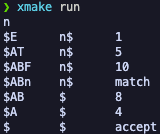
\includegraphics[width=\textwidth]{images/ll_1.png}
        \caption{LL(1)最简单的单个因子测试}
        \label{fig:ll-1}
    \end{minipage}
    \begin{minipage}[t]{0.3\textwidth}
        \centering
        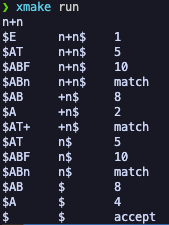
\includegraphics[width=\textwidth]{images/ll_2.png}
        \caption{LL(1)简单的加法测试}
        \label{fig:ll-2}
    \end{minipage}
    \begin{minipage}[t]{0.3\textwidth}
        \centering
        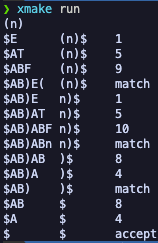
\includegraphics[width=\textwidth]{images/ll_3.png}
        \caption{LL(1)使用括号包裹单个表达式测试}
        \label{fig:ll-3}
    \end{minipage}
\end{figure}

\subsubsection{最简单的单个因子}
\paragraph{输入} $n$

仅有一个操作数,无操作符,测试程序对简单有效输入的处理。测试结果如~\autoref{fig:ll-1} 所示。

\subsubsection{简单的加法}
\paragraph{输入} $n+n$

测试程序对基本二元操作的处理。测试结果如~\autoref{fig:ll-2} 所示。

\subsubsection{使用括号包裹单个表达式}
\paragraph{输入} $(n)$

测试程序对带括号的简单表达式解析。测试结果如~\autoref{fig:ll-3} 所示。

\begin{figure}[htbp]
    \centering
    \begin{minipage}[t]{0.3\textwidth}
        \centering
        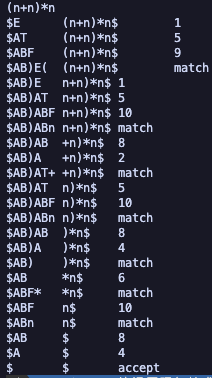
\includegraphics[width=\textwidth]{images/ll_4.png}
        \caption{LL(1)复杂度稍高,带括号与加法混合}
        \label{fig:ll-4}
    \end{minipage}
    \begin{minipage}[t]{0.3\textwidth}
        \centering
        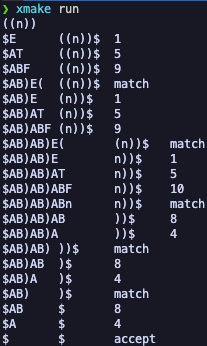
\includegraphics[width=\textwidth]{images/ll_5.png}
        \caption{LL(1)嵌套括号}
        \label{fig:ll-5}
    \end{minipage}
    \begin{minipage}[t]{0.3\textwidth}
        \centering
        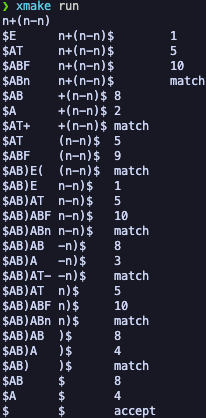
\includegraphics[width=\textwidth]{images/ll_6.png}
        \caption{LL(1)嵌套加减混合}
        \label{fig:ll-6}
    \end{minipage}
\end{figure}

\subsubsection{复杂度稍高,带括号与加法混合}
\paragraph{输入} $(n+n)*n$

测试括号内运算与外部运算的组合。测试结果如~\autoref{fig:ll-4} 所示。

\subsubsection{嵌套括号}
\paragraph{输入} $((n))$

测试多重括号嵌套的正确处理。测试结果如~\autoref{fig:ll-5} 所示。

\subsubsection{嵌套加减混合}
\paragraph{输入} $n+(n-n)$

测试嵌套的子表达式,以及在同一行处理加减混合运算。测试结果如~\autoref{fig:ll-6} 所示。

\begin{figure}[htbp]
    \centering
    \begin{minipage}[t]{0.3\textwidth}
        \centering
        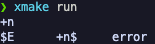
\includegraphics[width=\textwidth]{images/ll_7.png}
        \caption{LL(1)错误用例:表达式以操作符开头}
        \label{fig:ll-7}
    \end{minipage}
    \begin{minipage}[t]{0.3\textwidth}
        \centering
        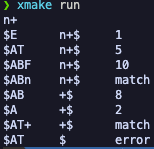
\includegraphics[width=\textwidth]{images/ll_8.png}
        \caption{LL(1)错误用例:表达式以操作符结尾}
        \label{fig:ll-8}
    \end{minipage}
    \begin{minipage}[t]{0.3\textwidth}
        \centering
        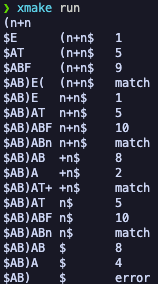
\includegraphics[width=\textwidth]{images/ll_9.png}
        \caption{LL(1)错误用例:缺少右括号}
        \label{fig:ll-9}
    \end{minipage}
\end{figure}

\subsubsection{错误用例:表达式以操作符开头}
\paragraph{输入} $+n$

表达式不符合文法规则,期望输出 \texttt{error}。测试结果如~\autoref{fig:ll-7} 所示。

\subsubsection{错误用例:表达式以操作符结尾}
\paragraph{输入} $n+$

不完整的表达式,缺少操作数,期望输出 \texttt{error}。测试结果如~\autoref{fig:ll-8} 所示。

\subsubsection{错误用例:缺少右括号}
\paragraph{输入} $(n+n$

缺失右括号,期望输出 \texttt{error}。测试结果如~\autoref{fig:ll-9} 所示。

通过以上测试用例,可以覆盖:\begin{compactitem}
	\item 基本的合法表达式(单一操作数、简单二元操作、多重操作)
	\item 带括号的复杂表达式
	\item 嵌套括号与嵌套表达式
	\item 非法输入(以操作符开头/结尾、括号不匹配)
\end{compactitem}

这些用例足以全面测试 LL(1) 预测分析程序的正确性和健壮性。

\section{编写 LR(1) 语法分析程序}

\subsection{题目要求}

\subsubsection{实验背景}
来自《编译原理与技术(第 2 版)》第 4 章的\textbf{程序设计 2}(方法 3)。

\subsubsection{任务描述}

编写一个语法分析程序,能对算数表达式进行 LR(1) 语法分析。

\paragraph{要求}对给定文法的产生式进行如下编号后:
\begin{table}[htbp]
    \centering
    \begin{tabular}{ll}
        \hline
        编号 & 产生式                \\ \hline
        0  & $E'\to E  $        \\
        1  & $E \to E+T$        \\
        2  & $E \to E-T$        \\
        3  & $E \to T  $        \\
        4  & $T \to T*F$        \\
        5  & $T \to T/F$        \\
        6  & $T \to F  $        \\
        7  & $F \to (E)$        \\
        8  & $F \to \text{num}$ \\
        10 & $F \to \text{num}$ \\ \hline
    \end{tabular}
\end{table}
\begin{compactenum}
    \item 编程实现构造该文法的 LR(1) 分析表。
    \item 编程实现算法 4.3,构造 LR(1) 分析程序。
\end{compactenum}

\subsubsection{编程要求}

根据注释提示,补充代码。
\paragraph{要求} 使用 C/C++ 实现

\paragraph{平台环境说明}
\begin{compactitem}
    \item 编译器版本:gcc \texttt{7.3.0}
    \item OS 版本:Debian GNU/Linux \texttt{9}
\end{compactitem}

\subsubsection{测试说明}

\paragraph{输入格式} 从标准输入(使用 \cppinline{cin/scanf} 等输入)读入数据。

输入仅包含 1 行:\begin{compactitem}
    \item 第 1 行输入为一个算术表达式。构成该算术表达式的字符有:\{`\verb|n|', `\verb|+|', `\verb|-|', `\verb|*|', `\verb|/|', `\verb|(|', `\verb|)|' \}。
\end{compactitem}

\paragraph{输出格式} 输出到标准输出(使用 \cppinline{cout/printf} 等输出)中。

输出包括若干行 LR(1) 分析过程:

假设输出有 $n$ 行,则第 $i$ 行 $(1\leq i \leq n)$ 表示分析进行到第 $i$ 步,它的输出仅包含一个部分:\begin{compactitem}
    \item 分析动作:归约使用的产生式编号或 \texttt{shift} 或 \texttt{error} 或 \texttt{accept}(表示当前步骤应执行的动作)
\end{compactitem}

注:规定第 1 步的分析过程为:根据分析栈中只有状态 0、输入串栈顶为第一个输入字符,来产生分析动作。

\subsection{程序设计说明}

求取 FIRST 集即之前的方法与代码与 LL(1) 分析程序类似,不再赘述。

\subsubsection{构造 closure($I$)}
伪代码如~\autoref{alg:closure} 所示。
\begin{algorithm}[htbp]
    \caption{构造 $\text{closure}(I)$ 的过程}
    \label{alg:closure}
    \KwIn{项目集合 $I$}
    \KwOut{$J = \text{closure}(I)$}
    
    $J \leftarrow I$\;
    \Repeat{$J_{\text{new}} = J$}{
        $J_{\text{new}} \leftarrow J$\;
        \ForEach{$[A \to \alpha \cdot B\beta, a] \in J_{\text{new}}$}{
            \ForEach{$B \to \eta$ 为文法 $G$ 中的产生式}{
                \ForEach{$b \in \mathrm{FIRST}(\beta a)$}{
                    \If{$[B \to \cdot \eta, b] \notin J$}{
                        将 $[B \to \cdot \eta, b]$ 加入 $J$\;
                    }
                }
            }
        }
    }
\end{algorithm}

由此实现 \cppinline{closure(I)} 函数对项目集 $I$ 不断添加满足 $[A \to \alpha \cdot B \beta, a]$ 的项目 $[B \to \cdot \gamma, b]$(其中 b 来自 FIRST($\beta a$))直至不再增加新项目。

\cppinline{goFunc(I, X)} 将 $I$ 中所有 $[A \to \alpha \cdot X\beta, a]$ 项目的 $dot$ 向右移动一位,变成 $[A \to \alpha X \cdot \beta, a]$,所得集合再取 closure。
\begin{cppcode}
std::set<Item> closure(const std::set<Item>& I)
{
    std::set<Item> J = I;
    bool changed = true;
    while (changed) {
        changed = false;
        std::set<Item> Jnew = J;
        for (const auto& it : J) {
            if (it.dot < static_cast<int>(it.right.size())) {
                char B = it.right[it.dot];
                if (nonterminals.count(B) != 0U) {
                    std::string beta = it.right.substr(it.dot + 1);
                    beta.push_back(it.lookahead);
                    std::set<char> firstSet = FIRST_str(beta);
                    if (firstSet.empty()) {
                        firstSet.insert(it.lookahead);
}
                    for (auto& p : prods) {
                        if (p.second.first == std::string(1, B)) {
                            for (auto b : firstSet) {
                                Item newItem = { p.second.first, p.second.second, 0, b };
                                if (J.count(newItem) == 0U) {
                                    Jnew.insert(newItem);
                                }
                            }
                        }
                    }
                }
            }
        }
        if (Jnew.size() != J.size()) {
            J = Jnew;
            changed = true;
        }
    }
    return J;
}

std::set<Item> goFunc(const std::set<Item>& I, char X)
{
    std::set<Item> J;
    for (const auto& it : I) {
        if (it.dot < static_cast<int>(it.right.size()) && it.right[it.dot] == X) {
            J.insert({ it.left, it.right, it.dot + 1, it.lookahead });
        }
    }
    return closure(J);
}
\end{cppcode}

\subsubsection{构造 LR(1) 项目集规范族}
\begin{compactitem}
    \item 定义 \cppinline{Item} 类表示 LR(1) 项目,其包含 \cppinline{left}, \cppinline{right}, \cppinline{dot}, \cppinline{lookahead}。
	\item 初始项目集 $I_0$ 包含 [$E' \to \cdot E$, \verb|$|]。通过 \cppinline{closure()} 函数将该集合闭包扩展,得到 $I_0$。
	\item 利用 \cppinline{goFunc()} 函数对状态集进行扩展:
\end{compactitem}
对规范族中的每个项目集 $I$ 和每个可能的文法符号 $X$,计算 $go(I, X)$。

若得到的新项目集不在规范族中,则加入规范族,直到不再增加新集合。算法如~\autoref{alg:lr1-canonical-collection} 所示。
\begin{algorithm}[htbp]
    \caption{构造文法 $G$ 的 LR(1) 项目集规范族}
    \label{alg:lr1-canonical-collection}
    \KwIn{文法 $G$}
    \KwOut{$G$ 的 LR(1) 项目集规范族 $C$}
    
    $C \leftarrow \{\mathrm{closure}(\{[S' \to \cdot S,\ \$]\})\}$\;
    
    \Repeat{无新项目集加入 $C$}{
        \ForEach{$I \in C$}{
            \ForEach{文法符号 $X$}{
                \If{$\mathrm{go}(I, X) \neq \emptyset$ 且 $\mathrm{go}(I, X) \notin C$}{
                    将 $\mathrm{go}(I, X)$ 加入 $C$\;
                }
            }
        }
    }
\end{algorithm}

\cppinline{buildAutomaton()} 从 $I_0$ 开始,反复对所有状态集和可能符号应用 \cppinline{goFunc()} 构造整个 LR(1) 自动机(即项目集规范族与状态转换)。

将每个项目集分配一个状态号,用于构建 LR(1) 分析表时使用。
\begin{cppcode}
void buildAutomaton()
{
    std::set<Item> I0;
    I0.insert({ startSymbol, "E", 0, '$' });
    I0 = closure(I0);
    getIndex(I0);
    bool added = true;
    while (added) {
        added = false;
        int n = static_cast<int>(C.size());
        for (int i = 0; i < n; i++) {
            std::set<char> Xs;
            for (const auto& it : C[i]) {
                if (it.dot < static_cast<int>(it.right.size())) {
                    Xs.insert(it.right[it.dot]);
                }
            }
            for (auto X : Xs) {
                std::set<Item> g = goFunc(C[i], X);
                if (!g.empty()) {
                    int j = 0;
                    if (Cidx.find(g) == Cidx.end()) {
                        j = getIndex(g);
                        added = true;
                    } else {
                        j = Cidx[g];
}
                    if (terminals.count(X) != 0U) {
                        action[i][X] = "s" + std::to_string(j);
                    }
                    if (nonterminals.count(X) != 0U) {
                        goTable[i][X] = j;
                    }
                }
            }
        }
    }
}    
\end{cppcode}

\subsubsection{构建 LR(1) 分析表}
算法如~\autoref{alg:build-lr1-analysis-table} 所示。
\begin{algorithm}[htbp]
    \caption{构造文法 $G$ 的 LR(1) 分析表的伪代码}
    \label{alg:build-lr1-analysis-table}
    \KwIn{文法 $G$}
    \KwOut{LR(1) 分析表 $action$ 和 $goto$}
    \SetAlgoLined
    根据 $G$ 的开始符号 $S$,构造拓广文法 $G'$,加入新的开始符号 $S'$,添加产生式 $S' \to S$。

    $C \leftarrow \{\mathrm{closure}(\{[S' \to \cdot S,\ \$]\})\}$\;
    \Repeat{无新项目集加入 $C$}{
        \ForEach{$I \in C$}{
            \ForEach{文法符号 $X$}{
                $J \leftarrow go(I,X)$\;
                \If{$J \neq \emptyset$ 且 $J \notin C$}{
                    将 $J$ 加入 $C$\;
                }
            }
        }
    }
    
    \ForEach{$I_i \in C$}{
        \ForEach{$[A \to \alpha \cdot a \beta, b] \in I_i$}{
            \If{$a$ 为终结符号 且 $go(I_i,a) = I_j$}{
                $action[i,a] \leftarrow S_j$\;
            }
        }
        \ForEach{$[A \to \alpha \cdot, a] \in I_i$}{
            \If{$A \neq S'$}{
                设 $A \to \alpha$ 在原文法中编号为 $r$,$action[i,a] \leftarrow R_r$\;
            }
        }
        \If{$[S' \to S \cdot,\ \$] \in I_i$}{
            $action[i,\$] \leftarrow ACC$\;
        }
    
        \ForEach{非终结符号 $A$}{
            \If{$go(I_i,A) = I_j$}{
                $goto[i,A] \leftarrow j$\;
            }
        }
    }
    
    \ForEach{$i$}{
        \ForEach{符号 $X$(包括终结符号和非终结符号)}{
            \If{$action[i,X]$ 和 $goto[i,X]$ 均未设定}{
                标记 $action[i,X]$ 或 $goto[i,X]$ 为 $error$\;
            }
        }
    }
    
    初态为包含 $[S' \to \cdot S,\ \$]$ 的项目集对应的状态。
    \end{algorithm}

实现 \cppinline{buildActionGoto()} 函数:\begin{compactitem}
    \item 对每个状态 $i$:\begin{compactitem}
        \item 若存在项目 $[A \to \alpha \cdot a \beta, b]$ 且 $go(i, a) = j$ 且 $a$ 为终结符,则 $action[i, a] = shift j$。
        \item 若存在 $[A \to \alpha \cdot , a]$ 且 A 不是拓广文法的开始符号,则 $action[i, a] = reduce by A\to\alpha $。产生式编号从 $prods$ 中获得。
        \item 若 $[E' \to E\cdot, \$]$ 在某状态中出现,则 $action[i, \$] = accept$。
    \end{compactitem}
	\item 对非终结符 $A$ 若 $go(i, A) = j$ 则 $goto[i, A] = j$。
	\item 未定义的表项为 \texttt{error}。
\end{compactitem}
\begin{cppcode}
void buildActionGoto()
{
    for (int i = 0; i < static_cast<int>(C.size()); i++) {
        for (const auto& it : C[i]) {
            if (it.dot == static_cast<int>(it.right.size())) {
                if (it.left == startSymbol && it.lookahead == '$') {
                    action[i]['$'] = "acc";
                } else {
                    for (auto& p : prods) {
                        if (p.second.first == it.left && p.second.second == it.right) {
                            action[i][it.lookahead] = "r" + std::to_string(p.first);
                        }
                    }
                }
            }
        }
    }
    for (int i = 0; i < static_cast<int>(C.size()); i++) {
        for (const auto& t : terminals) {
            if (action[i].find(t) == action[i].end()) {
                action[i][t] = "err";
            }
        }
        action[i]['$'] = (action[i].find('$') == action[i].end()) ? "err" : action[i]['$'];
    }
}
\end{cppcode}

\subsubsection{LR 语法分析}

\cppinline{LRparse()} 函数通过状态栈(\cppinline{stateStack})和符号栈(\cppinline{symbolStack})进行分析,算法如~\autoref{alg:lr1-parsing} 所示。
\begin{algorithm}[htbp]
    \caption{LR 分析程序}
    \label{alg:lr1-parsing}
    \KwIn{文法 $G$ 的 LR 分析表 (action 和 goto),输入符号串 $\omega$}
    \KwOut{若 $\omega \in L(G)$,则输出 $\omega$ 的自底向上分析过程,否则报告错误}
    
    将初始状态 $S_0$ 压入状态栈,将符号栈置空\;
    将 $\omega\$ $ 放入输入缓冲区,并令 $ip$ 指向其第一个符号\;
    
    \Repeat{终止}{
        设 $S$ 为状态栈顶状态,$a$ 为 $ip$ 所指向的输入符号\;
        \uIf{$action[S, a] = \text{shift } S'$}{
            将 $a$ 压入符号栈\;
            将 $S'$ 压入状态栈\;
            $ip \leftarrow ip + 1$\;
        }
        \uElseIf{$action[S, a] = \text{reduce by } A \to \beta$}{
            从符号栈和状态栈中弹出 $|\beta|$ 个符号和状态\;
            设当前状态栈顶为 $S'$\;
            将 $A$ 压入符号栈\;
            将 $goto[S', A]$ 压入状态栈\;
            输出产生式 $A \to \beta$\;
        }
        \uElseIf{$action[S, a] = accept$}{
            \textbf{return}\;
        }
        \Else{
            \textbf{error()}\;
        }
    }
\end{algorithm}
\begin{compactitem}
    \item 初始化:状态栈压入 0 状态。输入串末尾加 \verb|$|。
	\item 重复:\begin{compactitem}
        \item 取栈顶状态 $S$ 和当前输入符号 $a$。
        \item 查看 $action[S, a]$:\begin{compactitem}
            \item 若为 $shift s$:推入符号 $a$ 和状态 $s$,前移输入指针。
            \item 若为 $reduce by A \to \beta$:弹出 $|\beta|$ 个符号及状态,查看当前栈顶状态 $S’$,然后压入 $A$ 及 $goto[S', A]$。输出产生式编号。
            \item 若为 \texttt{accept}:输出 \texttt{accept},结束分析。
            \item 若为 \texttt{error}:输出 \texttt{error},结束分析。
        \end{compactitem}
    \end{compactitem}
\end{compactitem}
\begin{cppcode}
void LRparse(const std::string& input)
{
    std::stack<int> stateStack;
    std::stack<char> symbolStack;
    stateStack.push(0);
    int ip = 0;
    bool done = false;
    while (!done) {
        int S = stateStack.top();
        char a = input[ip];
        std::string act = (action[S].find(a) != action[S].end()) ? action[S][a] : "err";
        if (act == "acc") {
            std::cout << "accept\n";
            done = true;
        } else if (act[0] == 's') {
            std::cout << "shift\n";
            int nxt = std::stoi(act.substr(1));
            symbolStack.push(a);
            stateStack.push(nxt);
            ip++;
        } else if (act[0] == 'r') {
            int prodNo = std::stoi(act.substr(1));
            std::string A = prods[prodNo].first;
            std::string B = prods[prodNo].second;
            int len = static_cast<int>(B.size());
            for (int i = 0; i < len; i++) {
                symbolStack.pop();
                stateStack.pop();
            }
            int S2 = stateStack.top();
            symbolStack.push(A[0]);
            stateStack.push(goTable[S2][A[0]]);
            std::cout << prodNo << "\n";
        } else {
            std::cout << "error\n";
            done = true;
        }
    }
}
\end{cppcode}

\subsection{测试报告}

采用与 LL(1) 同样的测试。

\begin{figure}[htbp]
    \centering
    \begin{minipage}[t]{0.2\textwidth}
        \centering
        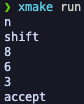
\includegraphics[width=\textwidth]{images/lr_1.png}
        \caption{LR(1)最简单的单个因子测试}
        \label{fig:lr-1}
    \end{minipage}
    \begin{minipage}[t]{0.2\textwidth}
        \centering
        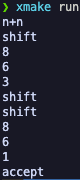
\includegraphics[width=\textwidth]{images/lr_2.png}
        \caption{LR(1)简单的加法测试}
        \label{fig:lr-2}
    \end{minipage}
    \begin{minipage}[t]{0.2\textwidth}
        \centering
        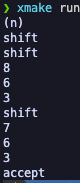
\includegraphics[width=\textwidth]{images/lr_3.png}
        \caption{LR(1)使用括号包裹单个表达式测试}
        \label{fig:lr-3}
    \end{minipage}
\end{figure}

\subsubsection{最简单的单个因子}
\paragraph{输入} $n$

仅有一个操作数,无操作符,测试程序对简单有效输入的处理。测试结果如~\autoref{fig:lr-1} 所示。

\subsubsection{简单的加法}
\paragraph{输入} $n+n$

测试程序对基本二元操作的处理。测试结果如~\autoref{fig:lr-2} 所示。

\subsubsection{使用括号包裹单个表达式}
\paragraph{输入} $(n)$

测试程序对带括号的简单表达式解析。测试结果如~\autoref{fig:lr-3} 所示。

\begin{figure}[htbp]
    \centering
    \begin{minipage}[t]{0.2\textwidth}
        \centering
        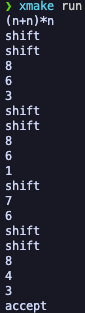
\includegraphics[width=\textwidth]{images/lr_4.png}
        \caption{LR(1)复杂度稍高,带括号与加法混合}
        \label{fig:lr-4}
    \end{minipage}
    \begin{minipage}[t]{0.2\textwidth}
        \centering
        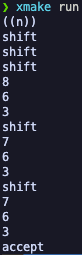
\includegraphics[width=\textwidth]{images/lr_5.png}
        \caption{LR(1)嵌套括号}
        \label{fig:lr-5}
    \end{minipage}
    \begin{minipage}[t]{0.2\textwidth}
        \centering
        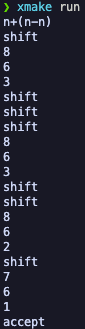
\includegraphics[width=\textwidth]{images/lr_6.png}
        \caption{LR(1)嵌套加减混合}
        \label{fig:lr-6}
    \end{minipage}
\end{figure}

\subsubsection{复杂度稍高,带括号与加法混合}
\paragraph{输入} $(n+n)*n$

测试括号内运算与外部运算的组合。测试结果如~\autoref{fig:lr-4} 所示。

\subsubsection{嵌套括号}
\paragraph{输入} $((n))$

测试多重括号嵌套的正确处理。测试结果如~\autoref{fig:lr-5} 所示。

\subsubsection{嵌套加减混合}
\paragraph{输入} $n+(n-n)$

测试嵌套的子表达式,以及在同一行处理加减混合运算。测试结果如~\autoref{fig:lr-6} 所示。

\begin{figure}[htbp]
    \centering
    \begin{minipage}[t]{0.2\textwidth}
        \centering
        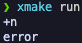
\includegraphics[width=\textwidth]{images/lr_7.png}
        \caption{LR(1)错误用例:表达式以操作符开头}
        \label{fig:lr-7}
    \end{minipage}
    \begin{minipage}[t]{0.2\textwidth}
        \centering
        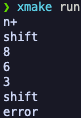
\includegraphics[width=\textwidth]{images/lr_8.png}
        \caption{LR(1)错误用例:表达式以操作符结尾}
        \label{fig:lr-8}
    \end{minipage}
    \begin{minipage}[t]{0.2\textwidth}
        \centering
        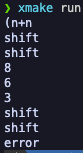
\includegraphics[width=\textwidth]{images/lr_9.png}
        \caption{LR(1)错误用例:缺少右括号}
        \label{fig:lr-9}
    \end{minipage}
\end{figure}

\subsubsection{错误用例:表达式以操作符开头}
\paragraph{输入} $+n$

表达式不符合文法规则,期望输出 \texttt{error}。测试结果如~\autoref{fig:lr-7} 所示。

\subsubsection{错误用例:表达式以操作符结尾}
\paragraph{输入} $n+$

不完整的表达式,缺少操作数,期望输出 \texttt{error}。测试结果如~\autoref{fig:lr-8} 所示。

\subsubsection{错误用例:缺少右括号}
\paragraph{输入} $(n+n$

缺失右括号,期望输出 \texttt{error}。测试结果如~\autoref{fig:lr-9} 所示。

全部符合预期。

\section{总结}

在完成 LL(1) 和 LR(1) 语法分析程序的设计与实现后,我深刻体会到编译原理中理论与实践结合的奥妙。这一过程不仅强化了我对语法分析基本原理的理解,也让我对设计和调试复杂算法的耐心与能力有了更高的要求。

首先,通过实现 LL(1) 分析程序,我进一步领会了自顶向下分析的核心思想——如何通过 FIRST 和 FOLLOW 集预测接下来的处理步骤。在构造预测分析表时,我遇到了文法消除左递归和提取公共左因子的问题。这些看似抽象的理论步骤,通过程序的实现和测试,变得清晰且有意义。同时,预测分析表的构建也让我感受到算法的精妙之处,尤其是如何在有限的上下文中高效确定下一步的行为。

接着,在实现 LR(1) 分析程序时,我切实体会到了自底向上分析的强大。相比 LL(1) 的局限性,LR(1) 能够处理更复杂的文法,这使得它的实现也更加繁琐。从项目集规范族的构建,到 closure 和 go 的细致处理,再到生成分析表的过程,每一步都充满了逻辑推导的挑战。尤其是 LR(1) 中对 lookahead 符号的管理,让我认识到它在消除语法歧义中的重要性。这部分的设计让我理解到,精确控制状态和转移,是解析复杂文法的关键。

在测试阶段,看到程序成功处理各种合法表达式,甚至能准确地报告错误时,那种成就感是难以言喻的。测试用例从简单到复杂,再到边界情况和错误输入,每个结果的正确输出都让我对理论的实用性和代码的可靠性感到欣慰。同时,这一过程也让我意识到测试的重要性——只有严谨的测试才能确保程序的健壮性。

此外,通过比较 LL(1) 和 LR(1) 的性能与适用性,我更深刻地理解了编译器的设计哲学——权衡简单性与能力。LL(1) 的实现相对简单,但对文法要求更高;而 LR(1) 虽然实现复杂,但适用范围广。这种取舍让我联想到工程实践中的实际决策,学会权衡理论上的完美与实际中的可行性。

总的来说,这次实验让我不仅收获了知识,还培养了分析问题和解决问题的能力。从理论到代码再到测试的完整闭环,让我更全面地理解了编译器的内部机制,也让我对后续深入学习和研究充满了信心。每一次调试,每一个测试结果,都是对编译原理魅力的最好诠释。

\appendix

\section{线上测试例通过情况截图}

\begin{figure}[htbp]
    \centering
    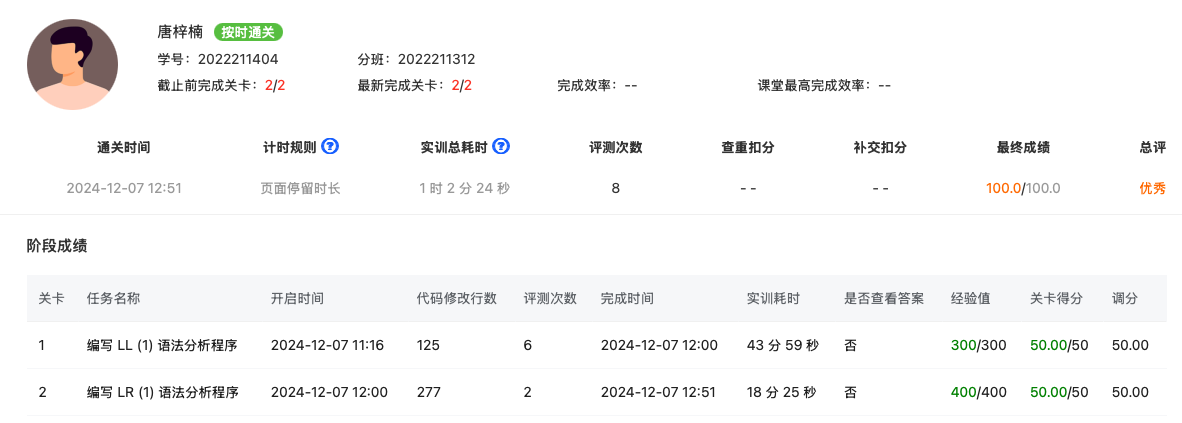
\includegraphics[width=0.9\textwidth]{images/pass.png}
\end{figure}